%!Mode:: "TeX:UTF-8"
\documentclass[a4paper,11pt,UTF8]{ctexart}

\usepackage{indentfirst} %缩进
\usepackage{xeCJK}    %使用系统字体
\usepackage{bm}       %粗体
\usepackage{fancyhdr} %自定义页眉页脚
\pagestyle{plain}                   %不设置页眉页脚
\usepackage{amsmath, amsthm, amssymb, amsfonts} %数学公式
\usepackage[a4paper,left=3cm,right=3cm,top=3.5cm,bottom=3.5cm]{geometry}
\usepackage{booktabs} %插入表格
\usepackage{diagbox}
\usepackage[section]{placeins} %避免浮动
\usepackage{listings} %插入代码
\usepackage{ctex}     %中文宏包
\usepackage[svgnames, table]{xcolor} %彩色表格
\usepackage{algorithm}          %伪代码
\usepackage{algorithmicx}
\usepackage{algpseudocode}
\usepackage{algorithm,algpseudocode,float}
\usepackage{lipsum}
\usepackage{enumitem}           %调整列举环境
\usepackage{url}
\usepackage{fontspec,xunicode}
\usepackage{subfigure}
\defaultfontfeatures{Mapping=tex-text} %如果没有它,会有一些 tex 特殊字符无法正常使用,比如连字符。

\usepackage{graphicx}
\graphicspath{{imgs/}}

%%%%%%%%%%%%%%%%%%%%%%%%%%%%%%%%%%%%%%%%%%%%%%%%%%%%%%%%%%%%%%%%
% 缩进及行间距
%%%%%%%%%%%%%%%%%%%%%%%%%%%%%%%%%%%%%%%%%%%%%%%%%%%%%%%%%%%%%%%%
\setlength{\parindent}{22bp} %重新定义缩进长度
\linespread{1}

%%%%%%%%%%%%%%%%%%%%%%%%%%%%%%%%%%%%%%%%%%%%%%%%%%%%%%%%%%%%%%%%
% 图的标题行间距设置
%%%%%%%%%%%%%%%%%%%%%%%%%%%%%%%%%%%%%%%%%%%%%%%%%%%%%%%%%%%%%%%%
\newcommand{\bottomcaption}{%
\setlength{\abovecaptionskip}{6bp}%
\setlength{\belowcaptionskip}{6bp}%
\caption}


%%%%%%%%%%%%%%%%%%%%%%%%%%%%%%%%%%%%%%%%%%%%%%%%%%%%%%%%%%%%%%%%
% 字体定义
%%%%%%%%%%%%%%%%%%%%%%%%%%%%%%%%%%%%%%%%%%%%%%%%%%%%%%%%%%%%%%%%
\setmainfont{Times New Roman}  %默认英文字体.serif是有衬线字体sans serif无衬线字体
\setmonofont{Consolas}
\setCJKmainfont[ItalicFont={楷体}, BoldFont={黑体}]{宋体}%衬线字体 缺省中文字体为
\setCJKsansfont{黑体}
\punctstyle{hangmobanjiao}
%-----------------------xeCJK下设置中文字体------------------------------%
\setCJKfamilyfont{song}{SimSun}                             %宋体 song
\newcommand{\song}{\CJKfamily{song}}
\setCJKfamilyfont{fs}{FangSong}                      %仿宋  fs
\newcommand{\fs}{\CJKfamily{fs}} 
\let\kaishu\relax                                    %重定义楷体,打开假粗体
\newCJKfontfamily\kaishu{KaiTi}[AutoFakeBold] 
%\setCJKfamilyfont{ktgb}{KaiTi_GB2312}                      %楷体 GB2312
%\newcommand{\ktgb}{\CJKfamily{ktgb}}
\setCJKfamilyfont{yh}{Microsoft YaHei}                    %微软雅黑 yh
\newcommand{\yh}{\CJKfamily{yh}}
\setCJKfamilyfont{hei}{SimHei}                              %黑体  hei
\newcommand{\hei}{\CJKfamily{hei}}
\setCJKfamilyfont{hwxk}{STXingkai}                                %华文行楷  hwxk
\newcommand{\hwxk}{\CJKfamily{hwxk}}
%------------------------------设置字体大小------------------------%
\newcommand{\chuhao}{\fontsize{42bp}{63bp}\selectfont}     %初号, 1.5倍行距
\newcommand{\xiaochuhao}{\fontsize{36bp}{36bp}\selectfont} %小初号,单倍行距
\newcommand{\yihao}{\fontsize{26bp}{39bp}\selectfont}        % 一号, 1.5 倍行距
\newcommand{\erhao}{\fontsize{22bp}{33bp}\selectfont}        % 二号, 1.5倍行距
\newcommand{\xiaoerhao}{\fontsize{18bp}{18bp}\selectfont}       % 小二, 单倍行距
\newcommand{\sanhao}{\fontsize{16bp}{24bp}\selectfont}       % 三号, 1.5倍行距
\newcommand{\xiaosanhao}{\fontsize{15bp}{22bp}\selectfont}      % 小三, 1.5倍行距
\newcommand{\sihao}{\fontsize{14bp}{21bp}\selectfont}        % 四号, 1.5 倍行距
\newcommand{\banxiaosi}{\fontsize{13bp}{20bp}\selectfont}  % 半小四, 20pt行距
\newcommand{\xiaosihao}{\fontsize{12bp}{20bp}\selectfont}       % 小四, 20pt行距
\newcommand{\dawuhao}{\fontsize{11bp}{11bp}\selectfont}      % 大五号, 单倍行距
\newcommand{\wuhao}{\fontsize{10.5bp}{10.5bp}\selectfont}   % 五号, 单倍行距
\newcommand{\xiaowuhao}{\fontsize{9bp}{9bp}\selectfont}   %小五号,单倍行距
%------------------------------重定义normalize------------------------%
\renewcommand{\normalsize}{\fontsize{12bp}{20bp}\selectfont}


%%%%%%%%%%%%%%%%%%%%%%%%%%%%%%%%%%%%%%%%%%%%%%%%%%%%%%%%%%%%%%%%
% 图题字体大小相同
%%%%%%%%%%%%%%%%%%%%%%%%%%%%%%%%%%%%%%%%%%%%%%%%%%%%%%%%%%%%%%%%
\usepackage{caption}
\captionsetup{font={footnotesize}}   % footnotesize = 9bp
\captionsetup[lstlisting]{font={footnotesize}}

%%%%%%%%%%%%%%%%%%%%%%%%%%%%%%%%%%%%%%%%%%%%%%%%%%%%%%%%%%%%%%%%
% 重定义枚举编号为 1),2)...
%%%%%%%%%%%%%%%%%%%%%%%%%%%%%%%%%%%%%%%%%%%%%%%%%%%%%%%%%%%%%%%%
\renewcommand{\labelenumi}{\theenumi)}


%%%%%%%%%%%%%%%%%%%%%%%%%%%%%%%%%%%%%%%%%%%%%%%%%%%%%%%%%%%%%%%%
% 重定义section标题
%%%%%%%%%%%%%%%%%%%%%%%%%%%%%%%%%%%%%%%%%%%%%%%%%%%%%%%%%%%%%%%%
\CTEXsetup[format={\CJKfamily{zhhei}\zihao{4}},number={\chinese{section}},name={,、~},aftername={},indent={0bp},beforeskip={6bp},afterskip={6bp},format+={\flushleft}]{section}
% \CTEXsetup[format={\Large\bfseries\CJKfamily{zhkai}\zihao{5}},name={(,)},number={\chinese{subsection}},aftername={},indent={22bp},beforeskip={6bp},afterskip={6bp}]{subsection}
\CTEXsetup[number={\chinese{section}},name={附录, ~~ }]{appendix}



%%%%%%%%%%%%%%%%%%%%%%%%%%%%%%%%%%%%%%%%%%%%%%%%%%%%%%%%%%%%%%%%
% 标题名称中文化
%%%%%%%%%%%%%%%%%%%%%%%%%%%%%%%%%%%%%%%%%%%%%%%%%%%%%%%%%%%%%%%%
\renewcommand\figurename{\hei 图}
\renewcommand\tablename{\hei 表}
\renewcommand\lstlistingname{\hei 代码}
\renewcommand{\algorithmicrequire}{\textbf{输入:}}
\renewcommand{\algorithmicensure}{\textbf{输出:}}
\newtheorem{define}{定义}


%%%%%%%%%%%%%%%%%%%%%%%%%%%%%%%%%%%%%%%%%%%%%%%%%%%%%%%%%%%%%%%%
% 列表设置
%%%%%%%%%%%%%%%%%%%%%%%%%%%%%%%%%%%%%%%%%%%%%%%%%%%%%%%%%%%%%%%%
\setlist[enumerate,1]{itemindent=22bp,listparindent=\parindent,itemsep=0mm,partopsep=.7mm,parsep=0ex,labelsep=1.5mm,topsep=0.7mm}
\setlist[enumerate,2]{label=\alph*),leftmargin=1.5em}  %二级item设置
%\setitemize{itemindent=38bp,leftmargin=0bp,itemsep=-0.4ex,listparindent=26bp,partopsep=0bp,parsep=0.5ex,topsep=-0.25ex}
%\setdescription{itemindent=38bp,leftmargin=0bp,itemsep=-0.4ex,listparindent=26bp,partopsep=0bp,parsep=0.5ex,topsep=-0.25ex}

%%%%%%%%%%%%%%%%%%%%%%%%%%%%%%%%%%%%%%%%%%%%%%%%%%%%%%%%%%%%%%%%
% 代码设置
%%%%%%%%%%%%%%%%%%%%%%%%%%%%%%%%%%%%%%%%%%%%%%%%%%%%%%%%%%%%%%%%
\lstset{
 columns=fixed,
 numbers=left,                                        % 在左侧显示行号
 numberstyle=\tiny\color{gray},                       % 设定行号格式
 frame=single,                                        % 单线背景边框
 breaklines=true,                                     % 设定LaTeX对过长的代码行进行自动换行
 keywordstyle=\color[RGB]{40,40,255},                 % 设定关键字颜色
 numberstyle=\footnotesize\color{darkgray},
 commentstyle=\it\color[RGB]{0,96,96},                % 设置代码注释的格式
 stringstyle=\rmfamily\slshape\color[RGB]{128,0,0},   % 设置字符串格式
 showstringspaces=false,                              % 不显示字符串中的空格
 language=java,                                        % 设置语言
 basicstyle=\linespread{1.0}\xiaowuhao\ttfamily,                      % 字体字号
 %lineskip=10bp,
 %baselinestretch=1,
}

%%%%%%%%%%%%%%%%%%%%%%%%%%%%%%%%%%%%%%%%%%%%%%%%%%%%%%%%%%%%%%%%
% 伪代码分页
%%%%%%%%%%%%%%%%%%%%%%%%%%%%%%%%%%%%%%%%%%%%%%%%%%%%%%%%%%%%%%%%
\makeatletter
\renewcommand{\ALG@name}{算法}
\newenvironment{breakablealgorithm}
  {% \begin{breakablealgorithm}
   \begin{center}
     \refstepcounter{algorithm}% New algorithm
     \hrule height.8bp depth0bp \kern2bp% \@fs@pre for \@fs@ruled
     \renewcommand{\caption}[2][\relax]{% Make a new \caption
       {\raggedright\textbf{\ALG@name~\thealgorithm} ##2\par}%
       \ifx\relax##1\relax % #1 is \relax
         \addcontentsline{loa}{algorithm}{\protect\numberline{\thealgorithm}##2}%
       \else % #1 is not \relax
         \addcontentsline{loa}{algorithm}{\protect\numberline{\thealgorithm}##1}%
       \fi
       \kern2bp\hrule\kern2bp
     }
  }{% \end{breakablealgorithm}
     \kern2bp\hrule\relax% \@fs@post for \@fs@ruled
   \end{center}
  }
\makeatother



\begin{document}
\xiaosihao\song

\begin{titlepage}
\center{\yihao{\hwxk{电子科技大学\underline{计算机科学与工程}学院}}}
\vspace{6cm}
\center{\xiaochuhao{\kaishu{\bfseries 实~验~报~告}}}
\vspace{4cm}

\begin{center}
\begin{large}
\begin{tabular}{rc}
\xiaoerhao{\hei{学\qquad 号}}& \hspace{1.7cm}\xiaoerhao{\hei{2020080903009\hspace{1.7cm}}} \\
\cline{2-2}\\
\xiaoerhao{\hei{姓\qquad 名}}& \xiaoerhao{\hei{李皓}}\\
\cline{2-2}\\
\xiaoerhao{\hei{(实验)课程名称}}& \xiaoerhao{\hei{MPI并行程序设计实验}}\\
\cline{2-2}\\
\xiaoerhao{\hei{教师}}& \xiaoerhao{\hei{卢国明}}\\
\cline{2-2}\\

\end{tabular}
\end{large}
\end{center}
\vfill \hfill
\end{titlepage}
\clearpage

\centerline{\\[10bp]\erhao{\fs{电 ~子 ~科~ 技~ 大~ 学}}}

\centerline{\\[20bp]\yihao{\fs{实  ~~~~ 验  ~~~~ 报  ~~~~ 告}}}

\leftline{\\[10bp]\sihao{\hei{\hspace{1.5em} 学生姓名:李皓 \hfill 学号:2020080903009 \hfill 指导教师:卢国明 }}}

% \leftline{\\[10bp]\sihao{\hei{\hspace{1.5em} 实验地点:信软楼西XXX \hfill }}}

% \leftline{\\[10bp]\sihao{\hei{\hspace{1.5em} 实验时间:第X周周X(X-X节) \hfill }}}

\setlength{\parskip}{0bp}  %定义段间距

\section{实验名称: MPI并行程序设计:埃氏素数筛选算法并行及性能优化}
% \section{实验学时: ~4}
\section{实验目的:}
\begin{enumerate}
  \item 使用MPI编程实现埃拉托斯特尼筛法并行算法。
  \item 对程序进行性能分析以及调优。
\end{enumerate}

\section{实验原理:}

埃拉托斯特尼是一位古希腊数学家,他在寻找整数$N$以内的素数时,采用了一种与众不同的方法:先将$2-N$的各数写在纸上:

在$2$的上面画一个圆圈,然后划去$2$的其他倍数;第一个既未画圈又没有被划去的数是$3$,将它画圈,再划去$3$的其他倍数;现在既未画圈又没有被划去的第一个数是$5$,将它画圈,并划去$5$的其他倍数……依此类推,一直到所有小于或等于$N$的各数都画了圈或划去为止。这时,画了圈的以及未划去的那些数正好就是小于$N$的素数。

这里,我们把$N$取$120$来举例说明埃拉托斯特尼筛法思想:

\begin{enumerate}
  \item 首先将$2$到$120$写出
  \item 在$2$上面画一个圆圈,然后划去$2$的其它倍数,这时划去的是除了$2$以外的其它偶数
  \item 从$2$往后一个数一个数地去找,找到第一个没有被划去的数$3$,将它画圈,再划去$3$的其它倍数(以斜线划去)
  \item 再从$3$往后一个数一个数地去找,找到第一个没有被划去的数$5$,将它画圈,再划去$5$的倍数(以交叉斜线划去)
  \item 再往后继续找,可以找到$9$、$11$、$13$、$17$、$19$、$23$、$29$、$31$、$37$、$41$、$43$、$47$,将它们分别画圈,并划去它们的倍数(可以看到,已经没有这样的数了)
  \item 这时,小于或者等于$120$的各数都画上了圈或者被划去,被画圈的就是素数了。
\end{enumerate}

\section{实验内容:}

\begin{enumerate}
  \item 完成Eratosthenes 筛法实现
  \item 进行并行程序的优化
  
  -安装部署 MPI 实验环境,并调试完成基准代码,实测在不同进程规模(1,2,4,8,16)加速比,并分析原因(40分)。

  -完成优化 1,去除偶数优化,实测在不同进程规模(1,2,4,8,16)加速比,并分析原因(10分)。

  -完成优化 2,消除广播优化,实测在不同进程规模(1,2,4,8,16)加速比,并分析原因(15分)。

  -完成优化 3,cache 优化,实测在不同进程规模(1,2,4,8,16)加速比,并分析原因(10分)。

  -在完成优化 3 的基础上,可以利用课内外知识,全面优化代码性能。根据班优化 3 在目标机上实测性能,最高性能(最短执行时间)得分 25 分,最低性能得 0 分,其他按执行时间进行插值。(25分)

\end{enumerate}

\section{实验设备:}

\begin{enumerate}
  \item 操作系统:Windows 11 专业版
  \item CPU: Ryzen 5-5700X
  \item 编程环境:vscode
  \item 执行环境:实验室服务器集群
  \item Node-CPU: Intel(R) Xeon(R) Gold 5318Y x2
\end{enumerate}
\section{实验步骤:}

\subsection{MPI 环境的配置和基本程序的运行}
在Windows上下载安装MPI程序,以及最新版本的vs stdio。随后进行环境变量的配置,以及新工程的创建。创建一个新的控制台应用,如下图所示:
\begin {figure}[h]
\centering % 居中显示
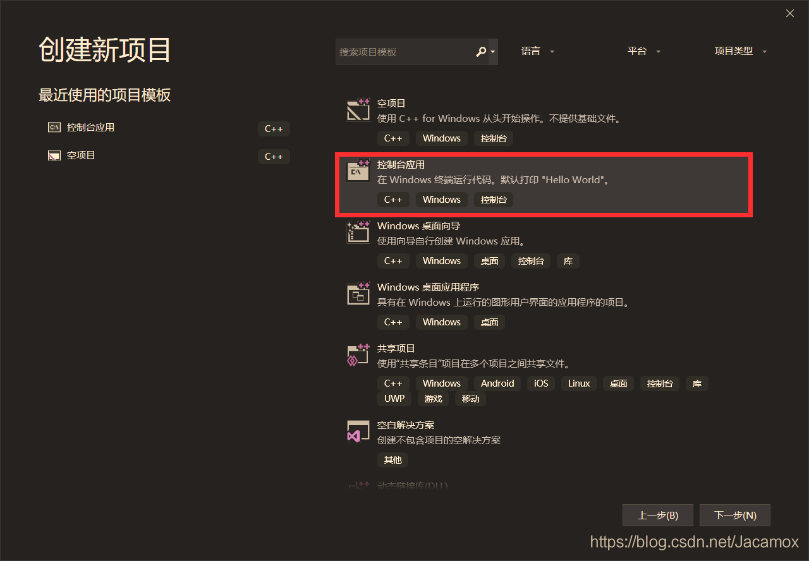
\includegraphics[width=0.7\textwidth]{3509-041319.png}
\caption{创建新的vs项目} % 标题
\label{five}
\end {figure}

\newpage
 随后进行环境变量和编译环境的设置,我们的素数筛选程序是一个MPI程序,因此运行时需要添加msmpi库的依赖,添加编译多线程运行的选项。完成上述配置后就可以将原始程序编译通过。

由于途中基准代码的部分变量是int类型,对于测试所需的$10^{10}$大小的数据可能存在溢出的风险。因此需要对原始的数据类型进行修改,如下所示:

\begin {figure}[h]
\centering % 居中显示
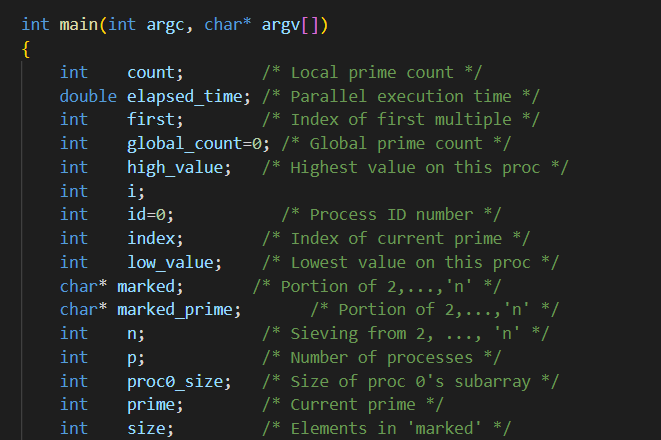
\includegraphics[width=0.5\textwidth]{4940-041319.png}
\caption{原始代码数据类型} % 标题
\label{five}
\end {figure}

使用int可能会造成溢出,导致结果计算的不正确,经过修改数据类型,以及分块计算的部分(图\ref{2})后即可编译运行,实测在不同进程规模(1,2,4,8,16)加速比。
\begin {figure}[h]
\centering % 居中显示
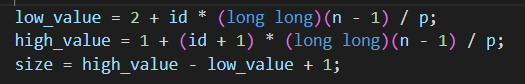
\includegraphics[width=0.5\textwidth]{5541-041319.png}
\caption{经过修改后的分块计算} % 标题
\label{five}
\end {figure}

\subsection{优化I:跳过偶数}

跳过偶数的思想主要是在于一个朴素的思想:偶数一定不是质数。对于我们的任务而言,计算$N$以内的素数个数,有大约$N/2$的数据不需要进行考虑。这一数据的减少,带来了存储数据的减少,因此需要对数据结构进行重构。在原始的算法中,用于标记素数的数组具有线性映射的关系,正如图(\ref{2})所示。而现在的数组和实际的素数构成了一个带有倍数关系的映射,原数据从3开始考虑素数的个数,这个数映射到mask的第0号。由于素数不予考虑,数字5映射到数组的第1位。

根据以上的映射关系,我们构造了从实际序数(ODD)到序号(index)的映射。为了计算的方便,使用宏定义的方式对运算进行替换:
\begin{lstlisting}[language=C++]
  #define ODD_TO_INDEX(odd) (((odd)-3)/2)     
  #define INDEX_TO_ODD(index) (2*(index)+3)   //对序号进行转换
\end{lstlisting}

在经过以上转换后,涉及mask数组的访问就使用index来进行,主要是进行下面的修改:

\begin{enumerate}
  \item 对于搜寻素数的操作进行重构:
  
  改动包括但是不限于将开始的素数由改为3,对循环中的判断操作转化为INDEX的大小比较。改动后的核心代码如下:
  \begin{lstlisting}[language=C++]
    if (!id) index = 0;
    prime = 3;
    do {
        if (prime * prime > low_value)
            first = ODD_TO_INDEX( prime * prime) -ODD_TO_INDEX( low_value);
            // 从prime*prime 开始找,因为(prime-1)之前的因数已经找过了
            // 对于分段后的数据而言,是先前一段的内容都被找到了
        else {
            if (!(low_value % prime)) 
                first = 0;
            // 如果开始的数就是因子的整数倍,那么就从这个开始找
            else {
                first = prime - (low_value % prime);
                if (!((low_value + first)%2)) 
                    first += prime;           
                    // 跳过偶数
                first /= 2;
                // 映射回index
            }
            // 如果不是,则为prime - (low_value % prime)
            // 假设 low_value 是 10 ,prime 为 3
            // first 就是 3-1= 2
            // 对应的就是mark[2]的位置,也就是 10,11,[12] 处
        }
        for (i = first; i < size; i += prime) marked[i] = 1;
        if (!id) {
            while (marked[++index]);
            // 找到下一个素数因子
            prime = INDEX_TO_ODD(index);
            // 从映射回序数
            // malloc 中的内容是从 0 开始索引,计算素数从2 开始。
        }
        if (p > 1) MPI_Bcast(&prime, 1, MPI_INT, 0, MPI_COMM_WORLD);
    } while (prime * prime <= n);
  \end{lstlisting}

  \item 对计数进行修正,由于计算素数个数时忽略所有二的倍数,包括2本身。因此在最后输出的时候需要+1。
  
\end{enumerate}

\subsection{优化II:取消并行通信}
根据课堂的知识:计算过程的并行开销是制约并行程序发展的瓶颈。在原始的代码中,只有0号进程计算了素数,向其余的进程广播之后,其余的进程才能够继续进行计算。期间的通信活动使得程序的并行性能不佳。因此我们对此处进行重构,为每个进程分配一个数组各自进行素数的计算。

主要的改动在于在原始的数组mask之外,再开一个数组marked\_prime来记录需要用到的素数。这个新开数组的大小只需$\sqrt{n}$。

在一个素数标记后,后续的更新不需进行进程的通信,只需要在素数数组中寻找下一个未标记数即可。

\subsection{优化III:cache优化}

cache 优化的思路类似于进行并行化的程序设计。也就是假设原始的数据规模为$n$经过划分后,分配给$p$个进程进行计算。那么每个进程获得了$n/p$的数据。在每个进程中,若需要优化性能,那么可以根据L3-cache的大小进行分段,将数据分为若干段,每一段都和cache的大小相符合。

在进行素数计算时,完成了一段cache的访问后,再整体读取下一段cache,这样可以极大优化程序的局部性,降低cache-miss的比例。

可以使用以下指令获取cache的大小:
\begin{lstlisting}[language=bash]
  getconf -a | grep CACHE
\end{lstlisting}

在实验室的机器上实验测得:
\newpage
\begin {figure}[h]
\centering % 居中显示
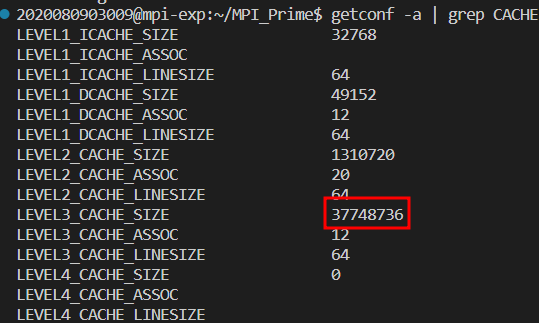
\includegraphics[width=0.5\textwidth]{5344-041320.png}
\caption{测试缓存指令} % 标题
\label{five}
\end {figure}
因此我们可以使用这一输出结果来确定数组分片的大小。

\subsection{优化IV:自由优化}
在上述的优化过程之外,我们还可以从以下的方法进行代码的重构和加速:
\begin{enumerate}
  \item 对素数数组的大小进行调整,使其更为精简。
  \item 考虑到计算时完成了许多序号到索引的转变,这些转变操作涉及到的乘法和除法可以换为更快的位移运算。
\end{enumerate}

以下为素数程序进行计算的流程图:
\begin {figure}[h]
\centering % 居中显示
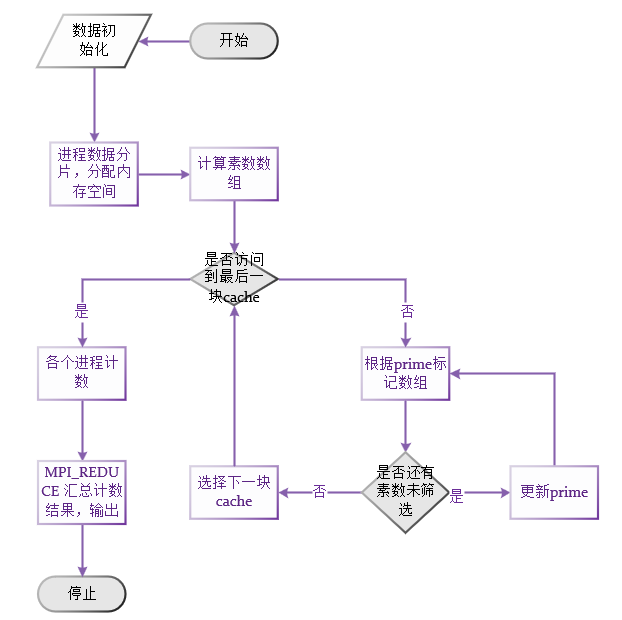
\includegraphics[width=\textwidth]{0242-041323.png}
\caption{埃氏素数筛法流程图} % 标题
\label{five}
\end {figure}


\section{实验结果与分析:}
\subsection{基准代码测试}
基准代码的加速比如下所示:\newpage
\begin{table}[ht]
\centering
\caption{不同进程数下,不同规模下的基准程序加速比}
\begin{tabular}{cccccccc}
  \toprule
  进程数$\backslash$ n & $10^3$             & $10^4$            & $10^5$           & $10^6$          & $10^7$          & $10^8$         & $10^9$         \\\midrule
  1   & \textbf{1}       & \textbf{1}       & \textbf{1}       & \textbf{1}       & \textbf{1}        & \textbf{1}        & \textbf{1}         \\
  2   & \textbf{0.13699} & \textbf{0.50813} & \textbf{1.14061} & \textbf{1.35139} & \textbf{1.930511} & \textbf{2.434571} & \textbf{1.7950923} \\
  4   & \textbf{0.10989} & \textbf{0.30488} & \textbf{1.37152} & \textbf{2.8547}  & \textbf{3.47912}  & \textbf{4.687211} & \textbf{2.9950464} \\
  8   & \textbf{0.0678}  & \textbf{0.29621} & \textbf{2.19395} & \textbf{6.40209} & \textbf{4.388913} & \textbf{8.180517} & \textbf{5.3209422} \\
  16  & \textbf{0.01372} & \textbf{0.13034} & \textbf{1.70304} & \textbf{10.6278} & \textbf{16.83087} & \textbf{12.67581} & \textbf{7.417538} \\\bottomrule
  \end{tabular}
\label{label}
  \end{table}
\begin {figure}[h]
\centering % 居中显示
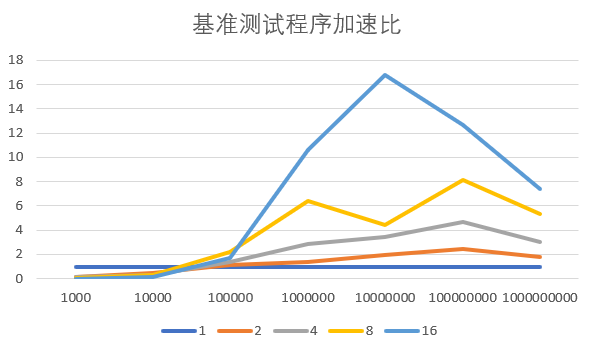
\includegraphics[width=\textwidth]{3535-041410.png}
\caption{基准程序加速比测试} % 标题
\label{five}
\end {figure}

分析该程序运行时的加速比可知,就整体趋势而言,加速比随着并行进程数量的增加而增加。在数字大小较小($<10^5$)时,由于任务本身不重,并行化开销比任务本身的串行开销要大,导致使用多线程时程序的加速比小于1。随着数据n规模的扩大,导致进程之间通信的开销增加,导致加速比回落,但是仍然保持在较高的水平。
\newpage
\subsection{优化I:跳过偶数}
以下为跳过偶数后的程序加速比。
\begin{table}[ht]
  \centering
  \caption{不同进程数下,不同规模下的跳过偶数后的加速比}
  \begin{tabular}{cccccccc}
    \toprule
    进程数$\backslash$ n & $10^3$             & $10^4$            & $10^5$           & $10^6$          & $10^7$          & $10^8$         & $10^9$         \\\midrule
    1   & \textbf{1}       & \textbf{1}       & \textbf{1}       & \textbf{1}       & \textbf{1}        & \textbf{1}        & \textbf{1}         \\
    2  & \textbf{0.076142} & \textbf{0.313636} & \textbf{0.978784} & \textbf{1.104057} & \textbf{1.806307} & \textbf{1.9402998} & \textbf{1.90209853} \\
    4  & \textbf{0.044379} & \textbf{0.146497} & \textbf{1.797403} & \textbf{2.819246} & \textbf{3.755661} & \textbf{3.5750619} & \textbf{2.55833746} \\
    8  & \textbf{0.038961} & \textbf{0.167883} & \textbf{1.303202} & \textbf{3.660101} & \textbf{7.735794} & \textbf{6.6292152} & \textbf{5.53268197} \\
    16 & \textbf{0.029644} & \textbf{0.069347} & \textbf{0.773184} & \textbf{3.779198} & \textbf{14.45695} & \textbf{12.497346} & \textbf{6.6352114} \\\bottomrule
    \end{tabular}
  \label{label}
    \end{table}
  \begin {figure}[h]
  \centering % 居中显示
  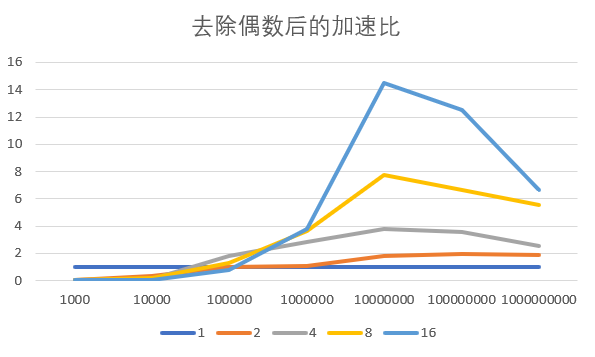
\includegraphics[width=\textwidth]{4502-041410.png}
  \caption{去除偶数后的加速比测试} % 标题
  \label{five}
  \end {figure}

与上一次进行对比可以发现,加速比的提升并不明显,而整体的趋势还是保持一致。这是由于消除偶数的行为只是去除了偶数,并且增加了一部分位置映射的计算,较之于并行开销而言,提升并不明显。但是在与基准代码的纵向对比中也可以看出,在同一运行条件下,优化I代码的运行时间平均只有基准代码的一半,带来了数值上的绝对提升。

\subsection{优化II:取消并行通信}
以下为取消并行通信后的程序加速比。
\begin{table}[ht]
  \centering
  \caption{不同进程数下,不同规模下的跳过进程通信后的加速比}
  \begin{tabular}{cccccccc}
    \toprule
    进程数$\backslash$ n & $10^3$             & $10^4$            & $10^5$           & $10^6$          & $10^7$          & $10^8$         & $10^9$         \\\midrule
    1   & \textbf{1}       & \textbf{1}       & \textbf{1}       & \textbf{1}       & \textbf{1}        & \textbf{1}        & \textbf{1}         \\
    2  & \textbf{0.714286} & \textbf{0.88}     & \textbf{1.005626} & \textbf{0.615108} & \textbf{1.840823} & \textbf{2.0596689} & \textbf{2.20605995} \\
    4  & \textbf{0.5}      & \textbf{1.54386}  & \textbf{2.344262} & \textbf{2.987882} & \textbf{3.920519} & \textbf{4.1683542} & \textbf{3.75156371} \\
    8 & \textbf{0.714286} & \textbf{1.833333} & \textbf{5.070922} & \textbf{6.341564} & \textbf{8.611069} & \textbf{8.556684} & \textbf{6.48140427} \\
    16 & \textbf{0.438596} & \textbf{0.473118} & \textbf{3.14978}  & \textbf{11.5}     & \textbf{13.20497} & \textbf{14.377272} & \textbf{9.16428213}\\\bottomrule
    \end{tabular}
  \label{label}
    \end{table}
  \begin {figure}[h]
  \centering % 居中显示
  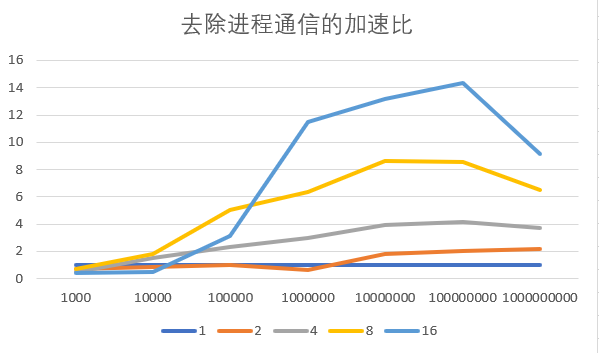
\includegraphics[width=\textwidth]{4854-041410.png}
  \caption{去除进程通信后的加速比} % 标题
  \label{five}
  \end {figure}

在去除并行通信后,并行通信就只有最后汇总计数的开销,通信的次数和数据量都在下降。反映到加速比可知:在n十分大的情况下,加速比的损失降低,这正是优化通信后的结果。
\newpage
\subsection{优化III:cache优化}

我们首先使用perf命令来查看优化II中cache的命中情况:
\begin {figure}[h]
\centering % 居中显示
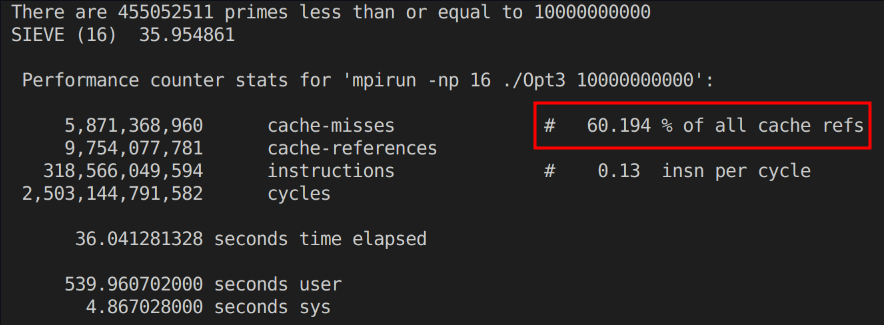
\includegraphics[width=\textwidth]{5031-041411.png}
\caption{优化II的cache-miss情况} % 标题
\label{five}
\end {figure}

由图可知,大约三分之二的cache都处于未命中的状态。这极大制约了程序的效率,我们对程序进行优化后得到以下的加速比:



\begin{table}[ht]
  \centering
  \caption{不同进程数下,不同规模下进行cache优化后的加速比}
  \begin{tabular}{cccccccc}
    \toprule
    进程数$\backslash$ n & $10^3$             & $10^4$            & $10^5$           & $10^6$          & $10^7$          & $10^8$         & $10^9$         \\\midrule
    1   & \textbf{1}       & \textbf{1}       & \textbf{1}       & \textbf{1}       & \textbf{1}        & \textbf{1}        & \textbf{1}         \\
    2  & \textbf{1.953856} & \textbf{1.433752} & \textbf{1.872933} & \textbf{1.936872} & \textbf{1.64537}  & \textbf{2.0102914} & \textbf{2.0628349}  \\
    4  & \textbf{1.982039} & \textbf{3.766319} & \textbf{3.759906} & \textbf{4.144591} & \textbf{4.085892} & \textbf{4.1677506} & \textbf{4.22854376} \\
    8  & \textbf{7.806353} & \textbf{8.564617} & \textbf{8.893048} & \textbf{9.547098} & \textbf{9.273755} & \textbf{8.9036151} & \textbf{8.62631875} \\
    16 & \textbf{5.42771}  & \textbf{17.11815} & \textbf{18.04168} & \textbf{19.0874}  & \textbf{6.868363} & \textbf{17.295912} & \textbf{16.7828432}\\\bottomrule
    \end{tabular}
  \label{label}
    \end{table}\newpage
  \begin {figure}[h]
  \centering % 居中显示
  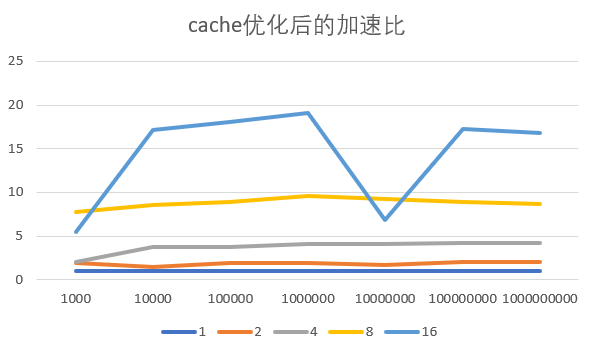
\includegraphics[width=\textwidth]{0628-041411.png}
  \caption{进行cache优化后的加速比测试} % 标题
  \label{five}
  \end {figure}

  可见优化后的程序局部性非常好,在部分p和n的组合下能够达到大于进程数量的加速比。其原因在于优化III限制了访问内存的范围不大于cache,对于计算机而言更有助于进行cache的刷新。由于计算机上不止一个进程在运行,cache的占用状态也有所不同。因此cache带来的加速效果也不稳定,在16个进程的情况下某次测试进程加速比有很大的波动。

\subsection{优化IV:自由优化}
进行自由优化后,程序的效率了显著提升:
\begin{table}[ht]
\centering
\caption{不同优化下的程序运行时间}
\begin{tabular}{ccccc}
\toprule
进程数$\backslash$ 优化& base              & 优化1               & 优化2               & 优化3               \\\midrule
$10^{9}$  & \textbf{1.654583} & \textbf{1.564225} & \textbf{1.501048} & \textbf{0.54903}  \\
$10^{10}$ & \textbf{23}       & \textbf{14.86948} & \textbf{14.06185} & \textbf{4.878388} \\ 

\bottomrule
  \end{tabular}
\label{label}
  \end{table}

  在同一运行条件下,优化3较之于基准代码快了近5倍,反映出对并行程序的合理设计的加速效果。

\section{总结及心得体会:}

在本次实验中,我基本掌握和复现了MPI并行程序设计的方法。并且通过四次程序的优化,直观认识了不同性能优化方法的效果以及特点。

经过这次实验我对并行程序设计的优化有了新的认识,在后续的实践中可以对这些技巧灵活应用。

\section{对本实验过程及方法、手段的改进建议:}
在实验时需要一些代码调优的工具,如perf和tau等,但是网上似乎没有相应的资源,导致瓶颈分析困难。

\vspace{4cm}
\begin{flushright}
\begin{tabular}{lc}
\sihao{\hei{报告评分:}}& \sihao{\vspace{10pt}}\\


\sihao{\hei{本人签字:}}&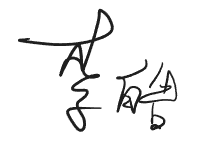
\includegraphics[width=60pt]{3341-041412.png}\\
\sihao{\hei{指导教师签字:}}& \sihao{\vspace{10pt}}\\

\end{tabular}
\end{flushright}

\newpage\section{代码清单}
\begin{enumerate}
  \item 代码I
  
  \lstinputlisting[language=C++,linewidth=\textwidth]{o1.cpp}
  \item 代码II
  
  \lstinputlisting[language=C++,linewidth=\textwidth]{o2}
  \item 代码III
  
  \lstinputlisting[language=C++,linewidth=\textwidth]{o3}
  \item 代码IV
  
  \lstinputlisting[language=C++,linewidth=\textwidth]{o4}
\end{enumerate}

\end{document}
